To investigate the efficacy of Roots as an approach to
implementing performance diagnostics as a PaaS service, we have developed a
working prototype, and a set of algorithms that uses it to automatically
identify SLO-violating performance anomalies.  For anomalies not caused by increases
in workload (HTTP request rate), Roots performs further analysis to identify the
bottleneck component that is responsible for the issue.

We implement our prototype in AppScale~\cite{6488671}, an open source PaaS cloud 
that is API compatible with Google App Engine (GAE)~\cite{gae}. This compatibility enables
us to evaluate our approach using real applications developed by others since
GAE applications run on AppScale without modification.
Because AppScale is open source,
we were able to modify its implementation minimally to integrate 
Roots. 

\begin{figure}
\centering
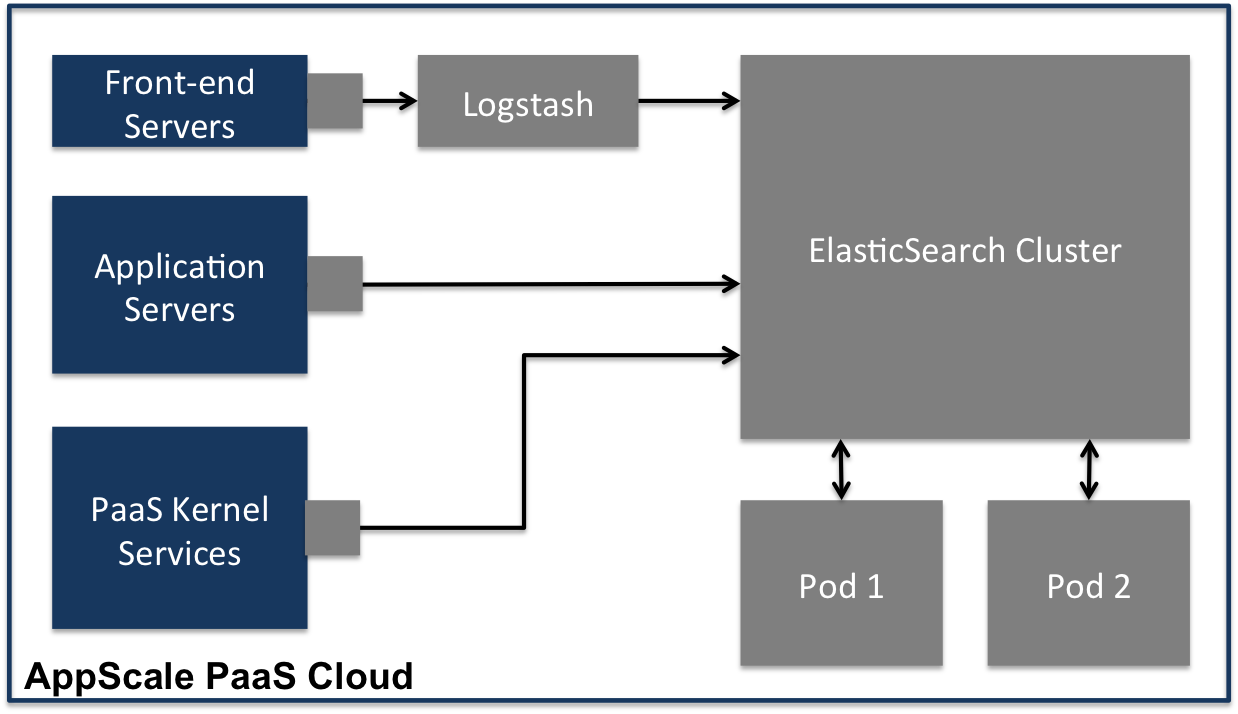
\includegraphics[scale=0.4]{roots_impl}
\caption{Roots prototype implementation for AppScale PaaS.}
\label{fig:roots_impl}
\end{figure}

Figure~\ref{fig:roots_impl} shows an overview of our prototype implementation. Roots components
are shown in grey, while the PaaS components are shown in blue.
We use ElasticSearch~\cite{elasticsearch} as the data storage component of our prototype. ElasticSearch is ideal 
for storing large volumes of structured and semi-structured data~\cite{Kononenko:2014:MMR:2597073.2597091}. 
%It supports scalability and high availability via sharding and replication.
ElasticSearch continuously organizes and indexes data, making the information available 
for fast and efficient querying. Additionally, it also provides
powerful data filtering and aggregation features, which greatly simplify the implementations of high-level
data analysis algorithms.

We configure AppScale's front-end server (based on Nginx) to tag all incoming application requests
with a unique identifier. This identifier is attached to the incoming request as a custom HTTP header.
All data collecting agents in the cloud extract this identifier, and include it as an attribute
in all the events reported to ElasticSearch. 
%This enables our prototype to aggregate events originating
%from the same application request.

We implement a number of data collecting agents in AppScale to gather runtime information
from all major components. These agents buffer data locally, and store them in ElasticSearch
in batches. Events are buffered until the buffer accumulates 1MB of data, subject to a hard time limit of 
15 seconds. This ensures that the events are promptly reported to the Roots data
storage while keeping the memory footprint of the data collecting agents small and bounded. 
For scraping server logs, and storing the extracted entries in ElasticSearch,
we use the Logstash tool~\cite{logstash}. 
%Logstash supports scraping a wide range of standard log formats (e.g. 
%Apache HTTPD access logs), and other custom log formats can be supported via a simple configuration.
%It also integrates naturally with ElasticSearch.
To capture the PaaS kernel invocation data, we augment AppScale's PaaS kernel implementation,
which is derived from the GAE PaaS SDK. More specifically we implement an agent that records
all PaaS SDK calls, and reports them to ElasticSearch asynchronously. 

We implement Roots pods as standalone Java server processes. Threads are used to run benchmarkers,
anomaly detectors and handlers concurrently within each pod. Pods communicate with ElasticSearch via
a web API, and many of the data analysis tasks such as filtering and aggregation are performed
in ElasticSearch itself. 
%This way, our Roots implementation offloads heavy computations 
%to ElasticSearch which is specifically designed for high-performance query processing
%and analytics. 
Some of the more sophisticated statistical analysis tasks (e.g. change point detection and 
linear regression as described below) are implemented in the R
language, and the Roots pods integrate with R using the Rserve protocol~\cite{Urbanek03rserve--}.
%Figure~\ref{fig:roots_impl} only shows two pods, but one can deploy an arbitrary number of pods to
%monitor the application load in the cloud platform.

\subsection{SLO-violating Anomalies}

As described previously,
Roots defines anomalies as performance events that trigger SLO
violations. Thus, we devise a detector to automatically identify when a SLO
violation has occurred. This anomaly detector
allows application developers to specify simple performance SLOs for deployed applications. A
performance SLO consists of an upper bound on the application response time ($T$), and the probability ($p$)
that the application response time falls under the specified upper bound. 
A general performance 
SLO can be stated as: ``application responds under $T$ milliseconds $p$\% of the time''.

When enabled for a given application, this anomaly detector starts a benchmarking process
that periodically measures the response time of the target application. Probes made by the benchmarking 
process are several seconds apart in time (sampling rate), so as to not strain the application with load.
The detector then periodically
analyzes the collected response time measurements to check if the application meets the specified performance
SLO. Whenever it detects that the application has failed to meet the SLO, it triggers an anomaly event. 
The SLO-based anomaly detector supports following configuration parameters:
\begin{itemize}
\item Performance SLO: Response time upper bound ($T$), and the probability ($p$).
\item Sampling rate: Rate at which the target application is benchmarked.
\item Analysis rate: Rate at which the anomaly detector checks whether the application has failed to meet the SLO.
\item Minimum samples: Minimum number of samples to collect before checking for SLO violations.
\item Window size: Length of the sliding window (in time) to consider when checking for SLO violations. This
acts as a limit on the number of samples to keep in memory.
\end{itemize}

%Once the anomaly detector identifies an SLO violation, it will continue to 
%identify the same violation
%until the historical data which contains the anomaly drops off from the sliding window. 
In order to prevent the detector from needlessly reporting the same anomaly multiple times,
we purge all the data from anomaly detector's sliding window whenever it detects an SLO violation.
Therefore, the detector cannot check for further SLO violations until it repopulates the sliding window 
with the minimum number of samples. This implies that each anomaly is followed by a ``warm up'' period.
For instance, with a sampling rate of 15 seconds, and a minimum
samples count of 100, the warm up period can last up to 25 minutes.

\subsection{Path Distribution Analysis}

We have implemented a path distribution analyzer
in Roots whose function it is to identify recurring sequences of
PaaS kernel invocations made by an application.
Each identified sequence corresponds to a path of
execution through the application code (i.e. a path through the control flow graph of the application). 
This detector is able to determine the frequency with
which each path is executed over time. Then, using this information which we term
a ``path distribution,'' it reports an anomaly event when the distribution of execution paths
changes. 

For each application,
a path distribution is comprised of the set of execution paths available in
that application, along with the proportion of requests that executed each path.
It is an indicator of the type of request workload handled by an application.
For example, consider a data management application that has a read-only execution path, and a read-write 
execution path. If 90\% of the requests execute the read-only path, and the remaining 10\% of the requests
execute the read-write path, we may characterize the request workload as read-heavy.

%
%is another special anomaly detector we implement in Roots. This
%anomaly detector periodically analyzes the PaaS kernel invocations made by the applications.
%By aggregating the PaaS kernel invocations by application request identifiers, and then sorting them by
%their sequence numbers, this anomaly detector is able to identify the sequence of
%PaaS kernel invocations made by each application request. 
%Each identified invocation sequence corresponds to a path of
%execution through the application code (i.e. a path through the control flow graph of the application). 
%Then the anomaly detector evaluates the number of requests
%that invoked the same PaaS kernel invocation sequence. From that the anomaly detector
%computes the distribution of different execution paths of an application.
 
Roots path distribution analyzer facilitates computing the path distribution for each application
with no static analysis, by only analyzing the runtime data gathered from the applications.
It periodically computes the path distribution for a given application.
If it detects that the latest path distribution is significantly different from the distributions seen in the 
past, it triggers an event. This is done by computing the mean request proportion for each path
(over a sliding window of historical data),
and then comparing the latest request proportion values against the means. If the latest proportion
is off by more than $n$ standard deviations from its mean, the detector considers it to be an
anomaly. The sensitivity of the detector can be configured by changing the value of $n$, which
defaults to 2. 

Path distribution analyzer enables developers to know when the nature of their application request
workload changes. For example in the previous data management application, if suddenly 90\%
of the requests start executing the read-write path, the Roots path distribution analyzer will
detect the change. Similarly it is also able to detect when new paths of execution
are being invoked by requests (a form of novelty detection).

\subsection{Workload Change Analyzer}

Performance anomalies can arise either due to bottlenecks in the cloud platform or 
changes in the application workload.
When Roots detects a performance anomaly (i.e. an application failing to meet its performance SLO),
it needs to be able to determine whether the failure is due
to an increase in workload or a bottleneck that has suddenly manifested.
To check if the workload of an application has changed recently, Roots uses a workload change analyzer.
This Roots component  is implemented as an anomaly handler, which gets executed every time an 
anomaly detector
identifies a performance anomaly. Note that this is different from the path distribution analyzer,
which is implemented as an anomaly detector. While the path distribution analyzer looks for changes in the
\textit{type} of the workload, the workload change analyzer looks for changes
in the workload \textit{size} or \textit{rate}. 
%In other words, it determines if the target application has received more requests than usual, which
%may have caused a performance degradation.

Workload change analyzer uses change point detection algorithms to analyze the historical trend of 
the application workload. We use the ``number of requests
per unit time'' as the metric of workload size. 
Our implementation of Roots supports a number of well known change point
detection algorithms (PELT~\cite{doi:10.1080/01621459.2012.737745}, binary segmentation 
and CL method~\cite{chen1993joint}), any of which can be used to detect level shifts in the
workload size. Algorithms like PELT favor long lasting shifts (plateaus) in the workload trend, over momentary spikes.
We expect momentary spikes to be fairly common in workload data. But it is the plateaus that cause
request buffers to fill up, and consume server-side resources for extended periods of time, thus
causing noticeable performance anomalies.

\subsection{Bottleneck Identification}
%The prototype Roots bottleneck identification algorithm uses a combination
%of quantile analysis, linear regression and change point detection. While Roots can
%support many different bottleneck identification algorithms, we use
%the algorithm proposed here in the experiments described below, and 
%find that it produces accurate results nearly 100\% of the time. It has been 
%designed to identify the true bottleneck from a number of candidates, and 
%we believe it to be a major contribution associated with this work.

Applications running in the cloud consist of user code executed in the application server, 
and remote service calls to various PaaS kernel services. An AppScale cloud
consists of the same kernel services present in the Google App Engine public cloud (datastore, memcache,
urlfetch, blobstore, user management etc.).
We consider each PaaS kernel invocation, and the code running on the application server as 
separate \textit{components}. Each application request causes one or more components to
execute, and any one of the components can become a bottleneck to cause performance anomalies.  
The purpose of bottleneck identification is to find, out of all
the components executed by an application, the one component that is most likely to have caused 
application performance to deteriorate.

Suppose an application makes $n$ PaaS kernel invocations ($X_1, X_2, ... X_n$) for each request. 
For any given application request,
Roots captures the time spent on each kernel invocation ($T_{X_1}, T_{X_2}, ... T_{X_n}$), and the 
total response time ($T_{total}$) of the request. These time values are related by the formula
$T_{total} = T_{X_1} + T_{X_2} + ... + T_{X_n} + r$, where $r$ is all the time spent in the resident 
application server executing user code (i.e. the time
spent not executing PaaS kernel services). $r$ is not
directly measured in Roots, since that requires code instrumentation.
However, in previous
work~\cite{Jayathilaka:2015:RTS:2806777.2806842} we showed that typical
PaaS-hosted web applications spend most of their time invoking PaaS kernel services.
We make use of these findings, and assert that for typical,
well-designed PaaS applications $r \ll T_{X_1} + T_{X_2} + ... + T_{X_n}$.

Roots bottleneck identification mechanism first
selects up to four components as possible candidates
for the bottleneck. These candidates are then further evaluated by a weighted algorithm to
determine the actual bottleneck in the cloud platform. 
%We begin by describing how Roots selects the four bottleneck candidates.

\subsubsection{Relative Importance of PaaS Kernel Invocations} 
The purpose of this metric is to find the component that is contributing 
the most towards the variance in the total response time. 
We select a window $W$ in time which includes a sufficient number of application requests,
and ending at the point when the performance anomaly was detected. Note that for each application request
in $W$, we can fetch the total response time ($T_{total}$), and the time spent on individual PaaS kernel
services ($T_{X_n}$) from the Roots data storage.
Then we take all the $T_{total}$ values
and the corresponding $T_{X_n}$ values in $W$, and fit 
a linear model of the form 
$T_{total} = T_{X_1} + T_{X_2} + ... + T_{X_n}$
using linear regression. Here we leave $r$ out
deliberately, since it is typically and ideally small. 

Occasionally in AppScale, we observe a request where $r$ is
large relative to $T_{X_n}$.  Often these events are correlated with large
$T_{X_n}$ values as well leading us to suspect that the effect may be due to
an issue with the AppScale infrastructure (e.g. a major garbage collection
event in the PaaS software).  Overall, Roots detects these events and identifies them correctly (cf
subsections~\ref{sec:highquantile} and ~\ref{sec:tailend} below), but they
perturb the linear regression model.  To prevent that,
we filter out requests where the $r$ value is too high. This
is done by computing the mean ($\mu_r$) and standard deviation ($\sigma_r$) of $r$ 
over the selected window, and removing 
any requests where $r > \mu_r + 1.65\sigma_r$.

Once the regression model has been computed, we run a relative importance algorithm~\cite{JSSv017i01} to rank each of the
regressors (i.e. $T_{X_n}$ values) based on their contribution to the variance of $T_{total}$. 
We use the LMG method~\cite{lmg80} which is resistant to multicollinearity, and provides a break down of the $R^2$ value of
the regression according to how strongly each regressor influences the variance of the dependent variable.
The relative importance values of the regressors add up to the $R^2$ of the linear regression. We consider
$1 - R^2$ (the portion of variance in $T_{total}$ not explained by the PaaS kernel invocations) as the relative importance of $r$. 
The component associated with the highest ranked regressor is chosen as a bottleneck candidate.
Statistically, this is the component that causes the application response time to vary the most.

\subsubsection{Changes in Relative Importance}
Next we divide the time window $W$ into equal-sized segments,
and compute the relative importance metrics for regressors within each segment. We also compute the
relative importance of $r$ within each segment. This way we can
obtain a time series of relative importance values for each regressor and $r$. These time series
represent how the relative importance of each component has changed over time.

We subject each relative importance time series to change point analysis to detect if the relative importance of any particular
variable has increased recently. If such a variable can be found, then the component
associated with that variable is also a potential candidate for the bottleneck. 
The candidate selected by this method represents
a component whose performance has been stable in the past, and has become variable recently. 

\subsubsection{High Quantiles}
\label{sec:highquantile}
Next we analyze the individual distributions of $T_{X_n}$ and $r$. 
%Recall that for each PaaS kernel invocation
%$X_k$, we have a distribution of $T_{X_k}$ values in the window $W$. Similarly we
%can also extract a distribution of $r$ values from $W$. 
Out of all the available distributions
we find the one whose quantile values are the largest.
Specifically, we compute a high
quantile (e.g. 0.99 quantile) for each distribution. The component, whose distribution 
contains the largest quantile value
is chosen as another potential candidate for the bottleneck. This component can be considered
having a high latency in general.

\subsubsection{Tail End Values}
\label{sec:tailend}
Finally, Roots analyzes each $T_{X_k}$ and $r$ distribution to identify the one 
with the largest tail values with respect to a particular high quantile.
For each maximum (tail end) latency value $t$, we compute the metric $P^q_t$ 
as the percentage difference between $t$ and a target quantile
$q$ of the corresponding distribution. We set $q$ to 0.99 in our experiments.
Roots selects the component with the 
distribution that has the largest $P^q_t$ as another potential bottleneck candidate.
This method identifies
candidates that contain rare, high-valued outliers (point anomalies) in their distributions.

\subsubsection{Selecting Among the Candidates}
The above four methods may select up to four candidate components for the bottleneck. 
We designate 
the candidate chosen by a majority of methods as the actual bottleneck. Ties
are broken by assigning more priority to the candidate chosen by the relative importance
method.